\documentclass{beamer}

% xcolor and define colors -------------------------
\usepackage{xcolor}

% https://www.viget.com/articles/color-contrast/
\definecolor{purple}{HTML}{5601A4}
\definecolor{navy}{HTML}{0D3D56}
\definecolor{ruby}{HTML}{9a2515}
\definecolor{alice}{HTML}{107895}
\definecolor{daisy}{HTML}{EBC944}
\definecolor{coral}{HTML}{F26D21}
\definecolor{kelly}{HTML}{829356}
\definecolor{cranberry}{HTML}{E64173}
\definecolor{jet}{HTML}{131516}
\definecolor{asher}{HTML}{555F61}
\definecolor{slate}{HTML}{314F4F}

% Mixtape Sessions
\definecolor{picton-blue}{HTML}{00b7ff}
\definecolor{violet-red}{HTML}{ff3881}
\definecolor{sun}{HTML}{ffaf18}
\definecolor{electric-violet}{HTML}{871EFF}

% Main theme colors
\definecolor{accent}{HTML}{00b7ff}
\definecolor{accent2}{HTML}{871EFF}
\definecolor{gray100}{HTML}{f3f4f6}
\definecolor{gray800}{HTML}{1F292D}


% Beamer Options -------------------------------------

% Background
\setbeamercolor{background canvas}{bg = white}

% Change text margins
\setbeamersize{text margin left = 15pt, text margin right = 15pt} 

% \alert
\setbeamercolor{alerted text}{fg = accent2}

% Frame title
\setbeamercolor{frametitle}{bg = white, fg = jet}
\setbeamercolor{framesubtitle}{bg = white, fg = accent}
\setbeamerfont{framesubtitle}{size = \small, shape = \itshape}

% Block
\setbeamercolor{block title}{fg = white, bg = accent2}
\setbeamercolor{block body}{fg = gray800, bg = gray100}

% Title page
\setbeamercolor{title}{fg = gray800}
\setbeamercolor{subtitle}{fg = accent}

%% Custom \maketitle and \titlepage
\setbeamertemplate{title page}
{
    %\begin{centering}
        \vspace{20mm}
        {\Large \usebeamerfont{title}\usebeamercolor[fg]{title}\inserttitle}\\
        {\large \itshape \usebeamerfont{subtitle}\usebeamercolor[fg]{subtitle}\insertsubtitle}\\ \vspace{10mm}
        {\insertauthor}\\
        {\color{asher}\small{\insertdate}}\\
    %\end{centering}
}

% Table of Contents
\setbeamercolor{section in toc}{fg = accent!70!jet}
\setbeamercolor{subsection in toc}{fg = jet}

% Button 
\setbeamercolor{button}{bg = accent}

% Remove navigation symbols
\setbeamertemplate{navigation symbols}{}

% Table and Figure captions
\setbeamercolor{caption}{fg=jet!70!white}
\setbeamercolor{caption name}{fg=jet}
\setbeamerfont{caption name}{shape = \itshape}

% Bullet points

%% Fix left-margins
\settowidth{\leftmargini}{\usebeamertemplate{itemize item}}
\addtolength{\leftmargini}{\labelsep}

%% enumerate item color
\setbeamercolor{enumerate item}{fg = accent}
\setbeamerfont{enumerate item}{size = \small}
\setbeamertemplate{enumerate item}{\insertenumlabel.}

%% itemize
\setbeamercolor{itemize item}{fg = accent!70!white}
\setbeamerfont{itemize item}{size = \small}
\setbeamertemplate{itemize item}[circle]

%% right arrow for subitems
\setbeamercolor{itemize subitem}{fg = accent!60!white}
\setbeamerfont{itemize subitem}{size = \small}
\setbeamertemplate{itemize subitem}{$\rightarrow$}

\setbeamertemplate{itemize subsubitem}[square]
\setbeamercolor{itemize subsubitem}{fg = jet}
\setbeamerfont{itemize subsubitem}{size = \small}


% Special characters

\usepackage{collectbox}

\makeatletter
\newcommand{\mybox}{%
    \collectbox{%
        \setlength{\fboxsep}{1pt}%
        \fbox{\BOXCONTENT}%
    }%
}
\makeatother





% Links ----------------------------------------------

\usepackage{hyperref}
\hypersetup{
  colorlinks = true,
  linkcolor = accent2,
  filecolor = accent2,
  urlcolor = accent2,
  citecolor = accent2,
}


% Line spacing --------------------------------------
\usepackage{setspace}
\setstretch{1.1}


% \begin{columns} -----------------------------------
\usepackage{multicol}


% Fonts ---------------------------------------------
% Beamer Option to use custom fonts
\usefonttheme{professionalfonts}

% \usepackage[utopia, smallerops, varg]{newtxmath}
% \usepackage{utopia}
\usepackage[sfdefault,light]{roboto}

% Small adjustments to text kerning
\usepackage{microtype}



% Remove annoying over-full box warnings -----------
\vfuzz2pt 
\hfuzz2pt


% Table of Contents with Sections
\setbeamerfont{myTOC}{series=\bfseries, size=\Large}
\AtBeginSection[]{
        \frame{
            \frametitle{Roadmap}
            \tableofcontents[current]   
        }
    }


% Tables -------------------------------------------
% Tables too big
% \begin{adjustbox}{width = 1.2\textwidth, center}
\usepackage{adjustbox}
\usepackage{array}
\usepackage{threeparttable, booktabs, adjustbox}
    
% Fix \input with tables
% \input fails when \\ is at end of external .tex file
\makeatletter
\let\input\@@input
\makeatother

% Tables too narrow
% \begin{tabularx}{\linewidth}{cols}
% col-types: X - center, L - left, R -right
% Relative scale: >{\hsize=.8\hsize}X/L/R
\usepackage{tabularx}
\newcolumntype{L}{>{\raggedright\arraybackslash}X}
\newcolumntype{R}{>{\raggedleft\arraybackslash}X}
\newcolumntype{C}{>{\centering\arraybackslash}X}

% Figures

% \imageframe{img_name} -----------------------------
% from https://github.com/mattjetwell/cousteau
\newcommand{\imageframe}[1]{%
    \begin{frame}[plain]
        \begin{tikzpicture}[remember picture, overlay]
            \node[at = (current page.center), xshift = 0cm] (cover) {%
                \includegraphics[keepaspectratio, width=\paperwidth, height=\paperheight]{#1}
            };
        \end{tikzpicture}
    \end{frame}%
}

% subfigures
\usepackage{subfigure}


% Highlight slide -----------------------------------
% \begin{transitionframe} Text \end{transitionframe}
% from paulgp's beamer tips
\newenvironment{transitionframe}{
    \setbeamercolor{background canvas}{bg=accent!40!black}
    \begin{frame}\color{accent!10!white}\LARGE\centering
}{
    \end{frame}
}


% Table Highlighting --------------------------------
% Create top-left and bottom-right markets in tabular cells with a unique matching id and these commands will outline those cells
\usepackage[beamer,customcolors]{hf-tikz}
\usetikzlibrary{calc}
\usetikzlibrary{fit,shapes.misc}

% To set the hypothesis highlighting boxes red.
\newcommand\marktopleft[1]{%
    \tikz[overlay,remember picture] 
        \node (marker-#1-a) at (0,1.5ex) {};%
}
\newcommand\markbottomright[1]{%
    \tikz[overlay,remember picture] 
        \node (marker-#1-b) at (0,0) {};%
    \tikz[accent!80!jet, ultra thick, overlay, remember picture, inner sep=4pt]
        \node[draw, rectangle, fit=(marker-#1-a.center) (marker-#1-b.center)] {};%
}

\usepackage{breqn} % Breaks lines

\usepackage{amsmath}
\usepackage{mathtools}

\usepackage{pdfpages} % \includepdf

\usepackage{listings} % R code
\usepackage{verbatim} % verbatim

% Video stuff
\usepackage{media9}

% packages for bibs and cites
\usepackage{natbib}
\usepackage{har2nat}
\newcommand{\possessivecite}[1]{\citeauthor{#1}'s \citeyearpar{#1}}
\usepackage{breakcites}
\usepackage{alltt}

% Setup math operators
\DeclareMathOperator{\E}{E} \DeclareMathOperator{\tr}{tr} \DeclareMathOperator{\se}{se} \DeclareMathOperator{\I}{I} \DeclareMathOperator{\sign}{sign} \DeclareMathOperator{\supp}{supp} \DeclareMathOperator{\plim}{plim}
\DeclareMathOperator*{\dlim}{\mathnormal{d}\mkern2mu-lim}
\newcommand\independent{\protect\mathpalette{\protect\independenT}{\perp}}
   \def\independenT#1#2{\mathrel{\rlap{$#1#2$}\mkern2mu{#1#2}}}
\newcommand*\colvec[1]{\begin{pmatrix}#1\end{pmatrix}}

\newcommand{\myurlshort}[2]{\href{#1}{\textcolor{gray}{\textsf{#2}}}}


\begin{document}

\imageframe{./lecture_includes/mixtape_did_cover.png}


% ---- Content ----

\section{Difference-in-Differences}

\subsection{Origins}


\begin{frame}{Introduction}

\begin{itemize}
\item Scott Cunningham, Ben H. Williams Professor of Economics at Baylor University in Texas USA
\item Today will talk about causal panel methods
\item Causal panel uses longitudinal data to estimate causal effects
\item We'll cover difference-in-differences and synthetic control methods
\end{itemize}

\end{frame}

\begin{frame}{Causal Inference vs Prediction}
  \centering
  \includegraphics[scale=0.5,height=6.5cm, width=10cm]{./lecture_includes/prediction_causality.png}
\end{frame}

\begin{frame}{Causal Inference vs Prediction}

  \begin{columns}
    \column{0.48\linewidth}
    \centering
    \textbf{Traditional prediction}
    \begin{itemize}
      \item Traditional prediction seeks to detect patterns in data and fit functional relationships between variables with a high degree of accuracy
      \item ``Does this person have heart disease?'', ``How many books will I sell?''
      \item It is not predictions of what effect a choice will have, though
    \end{itemize}
    \column{0.48\linewidth}
    \centering
    \textbf{Causal inference}
    \begin{itemize}
      \item Causal inference is also a type of prediction, but it's a prediction of a \emph{counterfactual} associated with a particular \emph{choice taken}
      \item Causal inference takes that predicted (or imputed) counterfactual and constructs a causal effect that we hope tells us about a future in the event of a similar choice taken
    \end{itemize}
  \end{columns}
\end{frame}








\begin{frame}{What is difference-in-differences (DiD)}

\begin{itemize}
\item DiD is when a group of units are assigned some treatment and then compared to a group of units that weren't before and after
\item One of the most widely used quasi-experimental methods in economics and increasingly in industry
\item Predates the randomized experiment by 80 years, but uses basic experimental ideas about treatment and control groups (just not randomized)
\item Uses panel or repeated cross section datasets, binary treatments usually, and often covariates
\item We'll do a quick run through the social history of diff-in-diff to set the stage for our workshop this week
\end{itemize}
\end{frame}








\begin{frame}{Ignaz Semmelweis and washing hands}

\begin{itemize}
\item Early 1820s, Vienna passed legislation requiring that if a pregnant women giving birth went to a public hospital (free care), then depending on the day of week and time of day, she would be routed to either the midwife wing or the physician wing (most likely resulting in random assignment)
\item But by the 1840s, Ignaz Semmelweis noticed that pregnant women died after delivery in the (male) wing at a rate of 13-18\%, but only 3\% in the (female) midwife wing -- cause was puerperal or “childbed” fever
\item Somehow this was also we known -- women would give birth in the street rather than go to the physician if they were unlucky enough to have their water break on the wrong day and time
\end{itemize}

\end{frame}

\begin{frame}{Ignaz Semmelweis and washing hands}

\begin{itemize}
\item Ignaz Semmelweis conjectures after a lot of observation that the cause is the teaching faculty teaching anatomy using cadavers and then delivering babies \emph{without washing hands}
\item New training happens to one but not the other and Semmelweis thinks the mortality is caused by working with cadavers
\item Convinced the hospital to have physicians wash their hands in chlorine but not the midwives, creating a type of difference-in-differences design 
\end{itemize}

\end{frame}

\begin{frame}{Semmelweis diff-in-diff evidence}

	\begin{figure}
	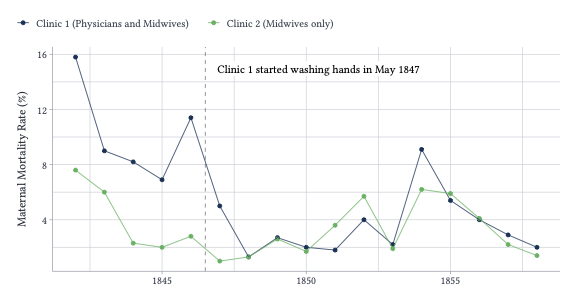
\includegraphics[scale=0.5]{./lecture_includes/semmelweis_raw_plots}
	\end{figure}


\end{frame}

\begin{frame}{Evidence Rejected}

\begin{itemize}

\item Diff-in-diff evidence was rejected by Semmelweis' superiors claiming it was the hospital's new ventilation system
\item Dominant theory of disease spread was caused by "odors" or miasma or "humors"
\item Semmelweis began showing signs of irritability, perhaps onset of dementia, became publicly abusive, was committed to a mental hospital and within two weeks died from wounds he received while in residence
\item Despite the strength of evidence, difference-in-differences was rejected -- a theme we will see continue

\end{itemize}

\end{frame}






\begin{frame}{John Snow and cholera}

\begin{itemize}
\item Three major waves of cholera in the early to mid 1800s in London, largely thought to be spread by miasma (``dirty air'')
\item John Snow believed cholera was spread through the Thames water supply through an invisible creature that entered the body through food and drink, caused the body to expel water, placing the creature back in the Thames and causing epidemic waves
\item London passes ordinance requiring water utility companies to move inlet pipe further up the Thames, above the city center, but not everyone complies
\item Natural experiment: Lambeth water company moves its pipe between 1849 and 1854; Southwark and Vauxhall water company delayed
\end{itemize}

\end{frame}




\begin{frame}

	\begin{figure}
	\caption{Two water utility companies in London 1854}
	\includegraphics[scale=0.225]{./lecture_includes/lambeth.png}
	\end{figure}


\end{frame}


\begin{frame}{Difference-in-differences}

\begin{table}\centering
\scriptsize
		\caption{Lambeth and Southwark and Vauxhall, 1849 and 1854}
		\begin{center}
		\begin{tabular}{lll|lc}
		\toprule
		\multicolumn{1}{l}{\textbf{Companies}}&
		\multicolumn{1}{c}{\textbf{Time}}&
		\multicolumn{1}{c}{\textbf{Outcome}}&
		\multicolumn{1}{c}{$D_1$}&
		\multicolumn{1}{c}{$D_2$}\\
		\midrule
		Lambeth & Before & $Y=L$ \\
		& After & $Y=L + L_t + D$ & $\textcolor{red}{L_t}+D$\\
		\midrule
		& & & & $D + (\textcolor{red}{L_t}- SV_t)$ \\
		\midrule
		Southwark and Vauxhall & Before & $Y=SV$ \\
		& After & $Y=SV + SV_t$ & $SV_t$\\
		\bottomrule
		\end{tabular}
		\end{center}
	\end{table}

\begin{eqnarray*}
\widehat{\delta}_{did} = D + (\textcolor{red}{L_t}- SV_t)
\end{eqnarray*}This method yields an unbiased estimate of D if $\textcolor{red}{L_t} = SV_t$, but note that $\textcolor{red}{L_t}$ is a counterfactual trend and therefore not known

\end{frame}





\begin{frame}
\begin{center}
\textbf{Two rivers into causal inference}
\end{center}

\begin{tikzpicture}[scale=0.7, every node/.style={scale=0.7}]
% Orley Ashenfelter Stream
\node at (-5,6) {\textbf{Orley Ashenfelter}};
\draw[->, thick] (-5,5.5) -- (-5,5.2);
\node at (-5,5) {Princeton Industrial Relations Section};
\draw[->, thick] (-5,4.5) -- (-5,4.2);
\node at (-5,4) {Quasi-Experimental Design};
\draw[->, thick] (-5,3.5) -- (-5,3.2);
\node at (-5,3) {David Card};
\draw[->, thick] (-5,2.5) -- (-5,2.2);
\node at (-5,2) {Alan Krueger};
\draw[->, thick] (-5,1.5) -- (-5,1.2);

% Don Rubin Stream
\node at (5,6) {\textbf{Don Rubin}};
\draw[->, thick] (5,5.5) -- (5,5.2);
\node at (5,5) {Harvard Statistics};
\draw[->, thick] (5,4.5) -- (5,4.2);
\node at (5,4) {Experimental Design};
\draw[->, thick] (5,3.5) -- (5,3.2);
\node at (5,3) {Potential Outcomes};
\draw[->, thick] (5,2.5) -- (5,2.2);
\node at (5,2) {Treatment Effects};
\draw[->, thick] (5,1.5) -- (5,1.2);

% Arrow from Orley Ashenfelter and Don Rubin streams to bottom rectangle
\draw[->, thick] (-5,1) -- (0,-0.8);
\draw[->, thick] (5,1) -- (0,-0.8);

% Bottom Rectangle
\node[draw, minimum width=8cm, minimum height=2cm, anchor=north] at (0,-0.8) {
    \begin{tabular}{c}
        Josh Angrist \\
        (Princeton)
    \end{tabular}
    \hspace{2cm}
    \begin{tabular}{c}
        Guido Imbens \\
        (Brown)
    \end{tabular}
};
\node[anchor=north] at (0,-2.8) {\textbf{Harvard Economics}};

\end{tikzpicture}

\end{frame}


\begin{frame}{Background I: Harvard Stats and Potential Outcomes}
  \begin{itemize}
    \item Don Rubin, former chair of Harvard stats, is the main source of potential outcomes, building on Jerzy Neyman's 1923 work.
    \item Rubin's influential 1970s papers advocated for causal inference using contrasts of $Y(1)$ and $Y(0)$.
    \item Neyman's notation, initially in Polish, was translated into English in 1990, likely due to Rubin.
    \item Rubin expanded Neyman's ideas from experiments to observational studies, leading to developments like propensity score methods.
    \item Economics was slow to adopt these methods initially.
  \end{itemize}
\end{frame}


\begin{frame}{Background II: Princeton Industrial Relations Section}
  \begin{itemize}
    \item Late 1970s and early 1980s: little "credibility" in empirical labor studies.
    \item Princeton Industrial Relations Section: older than the economics dept, rigorous, non-partisan focus on US "manpower", highly empirical.
    \item Key faculty are Orley Ashenfelter, David Card, Alan Krueger.
    \item Key students include Bob Lalonde, Josh Angrist, Steve Pischke, John Dinardo, Janet Currie, Anne Case, and many more.
    \item Listen to David Card: \url{https://youtu.be/1soLdywFb_Q?si=BCVqYeRz6jYiwHTQ&t=1580}
  \end{itemize}
\end{frame}


\begin{frame}{Background II: Princeton Industrial Relations Section}
Example of Princeton Paradigm Emerging
  \begin{itemize}
    \item Lalonde (1986) was a groundbreaking study, recently reviewed by Guido Imbens and Yiqing Xu (2024)
    \item Lalonde, a student of Card and Orley, analyzed an RCT on a job training program, finding an average treatment effect of +\$800.
    \item He then replaced the experimental control group with survey data, reran econometric methods, and couldn't replicate the results.
    \item Orley and Card emphasized randomization in their 1985 Restat article, advocating for its exploitation in studies.
  \end{itemize}
\end{frame}


\begin{frame}{Orley Ashenfelter and diff-in-diff}

\begin{itemize}

\item Diff-in-diff gets rediscovered by Orley Ashenfelter from Princeton 
\item Leaves academia to work in Washington DC to study job training programs for low skill workers
\item Coins the phrase "difference-in-differences" so as to avoid having to explain regressions to bureaucrats (3:53)  \url{https://youtu.be/WnB3EJ8K7lg?si=uE4clqUIPzvbxm0r&t=2}
\item More associated with David Card (Mariel boatlift, minimum wage), but it was earlier that he and Orley worked with the method, and ironically largely, rejected its usefulness for the questions they were working on

\end{itemize}

\end{frame}


\begin{frame}

\begin{itemize}
\item Card and Krueger (1994) have a famous study estimating causal effect of minimum wages on employment
\item  New Jersey raises its minimum wage in April 1992 (between February and November) but neighboring Pennsylvania does not
\item Using DiD, they do not find a negative effect of the minimum wage on employment leading to complex reactions from economists
\item Orley's describes his understanding of people's reaction to the paper.  \\ \url{https://youtu.be/MOtbuRX4eyQ?t=1882}
\end{itemize}

\end{frame}

\begin{frame}
	\begin{figure}
	\includegraphics[scale=0.5]{./lecture_includes/minwage_whore}
	\end{figure}
\end{frame}


\begin{frame}{Reaction to the paper}


Lots of anecdotes in this interview with Card, but here are just two.  First, Card and Krueger received a lot of personal hostility from their peers (1:07 to 1:10)

\bigskip

\url{https://youtu.be/1soLdywFb_Q?si=laAVYf_E2KBZKywG&t=4020}

\bigskip

Later Card says Sherwin Rosen accused them of having an agenda.  But the worst is what happens to Alan Krueger maybe (1:16 to 1:17)

\bigskip

\url{https://youtu.be/1soLdywFb_Q?si=jsb8h50ZosGDnKrv&t=4556}




\end{frame}

\begin{frame}{Card on that study}

\begin{quote}
``I’ve subsequently stayed away from the minimum wage literature for a number of reasons. First, it cost me a lot of friends. People that I had known for many years, for instance, some of the ones I met at my first job at the University of Chicago, became very angry or disappointed. They thought that in publishing our work we were being traitors to the cause of economics as a whole.''
\end{quote}


\end{frame}



\subsection{Potential outcomes}


\begin{frame}{Identification vs Estimation}

\begin{itemize}
\item We must start by making a distinction between the parameter we are attempting to identify and the manner in which we will estimate it
\item Identification requires first stating explicitly our goal expressed using potential outcomes
\item But often people skip this step and go directly to the numerical calculation like Orley was doing so let's do that

\end{itemize}

\end{frame}


\begin{frame}{Four Averages and Three Subtractions}
$$Y_{ist} = \alpha_0 + \alpha_1 Treat_{is} + \alpha_2 Post_{t} + \textcolor{blue}{\delta} (Treat_{is} \times Post_t) + \varepsilon_{ist} $$

\bigskip

$$\widehat{\textcolor{blue}{\delta}} = \bigg ( \overline{y}_k^{post(k)} - \overline{y}_k^{pre(k)} \bigg ) - \bigg ( \overline{y}_U^{post(k)} - \overline{y}_U^{pre(k)} \bigg ) $$

\begin{itemize}
\item Orley claims that the OLS estimator of $\delta$ and the ``four averages and three subtractions'' calculation are numerically identical \\ \url{https://youtu.be/WnB3EJ8K7lg?t=126}
\item They are and I want you to see that with a numerical example in \texttt{equivalence.do} and \texttt{equivalence.R}
\end{itemize}

\end{frame}

\begin{frame}{Introducing Potential Outcomes to DiD}

\begin{itemize}
\item Research question versus causal question -- not the same thing
\item Research question would be you are wanting to know effect of job training programs on earnings
\item Causal question is expressed using potential outcomes
\item Causal questions are usually averages of individual treatment effects for a specific population of units
\end{itemize}

\end{frame}




\begin{frame}{Potential outcomes notation}
	
	\begin{itemize}
	\item Let the treatment be a binary variable: $$D_{i,t} =\begin{cases} 1 \text{ if in job training program $t$} \\ 0 \text{ if not in job training program at time $t$} \end{cases}$$where $i$ indexes an individual observation, such as a person

	\end{itemize}
\end{frame}

\begin{frame}{Potential outcomes notation}
	
	\begin{itemize}

	\item Potential outcomes: $$Y_{i,t}^j =\begin{cases} 1 \text{: wages at time $t$ if trained} \\ 0 \text{: wages at time $t$ if not trained} \end{cases}$$where $j$ indexes a state of the world where the treatment happened or did not happen

	\end{itemize}
\end{frame}



\begin{frame}{Treatment effect definitions}


	\begin{block}{Individual treatment effect}
	    The individual treatment effect,  $\delta_i$, equals $Y_i^1-Y_i^0$
	\end{block}

Missing data problem:  No data on the counterfactual 
	
\end{frame}


\begin{frame}{Average Treatment Effects for the Treated Subpopulation}	
	\begin{block}{Average Treatment Effect on the Treated (ATT)}
	The average treatment effect on the treatment group is equal to the average treatment effect conditional on being a treatment group member:
		\begin{eqnarray*}
		E[\delta|D=1]&=&E[Y^1-Y^0|D=1] \nonumber \\
		&=&E[Y^1|D=1]-\textcolor{red}{E[Y^0|D=1]}
		\end{eqnarray*}
	\end{block}
	
	\bigskip

It's the average causal effect but only for the people exposed to some intervention; notice we can't calculate it, also, because we are missing the red term

	
\end{frame}

\begin{frame}{ATT vs ATE}

\begin{itemize}
\item Imagine there are 100 cities -- 25 of them raise the minimum wage, 75 do not
	\begin{itemize}
	\item ATE is the average treatment effect across all 100 cities
	\item ATT is the average treatment effect for the 25 cities that raised the minimum wage
	\end{itemize}
\item If you want to know the ATE, diff-in-diff is not appropriate as it only identifies the ATT
\item Just keep in mind the \emph{population} -- you can average the treatment effects for everyone or just some people, but whichever affects the interpretation
\end{itemize}

\end{frame}

\begin{frame}{Potential Outcomes vs Realized Outcomes}

\begin{itemize}
\item When you're analyzing data, you are working with the realized outcomes
\item When you are thinking about your treatment parameters, you are working with potential outcomes
\item When treatment does occur, then only one of the potential outcomes happens ("realized outcome") but the other one becomes "counterfactual" or missing
\item We represent this with the switching equation
 $$Y_{it}=D_{it}Y_{it}^1 + (1-D_{it})Y_{it}^0$$
\item How those treatment get assigned is called the treatment assignment mechanism, but let's review this together first before we discuss that

\end{itemize}
\end{frame}





\subsection{Assumptions and Estimation}


\begin{frame}{DiD equation is the 2x2}

Orley's ``four averages and three subtractions'' uses two groups, two time periods, or 2x2

\begin{eqnarray*}
\widehat{\delta} = \bigg ( E[Y_k|Post] - E[Y_k|Pre] \bigg ) - \bigg ( E[Y_U | Post ] - E[ Y_U | Pre] \bigg) \\
\end{eqnarray*}$k$ are the people in the job training program, $U$ are the untreated people not in the program, $Post$ is after the trainees took the class, $Pre$ is the period just before they took the class, and $E[y]$ is mean earnings. 

\bigskip

When will $\widehat{\delta}$ equal the ATT?  When will it not?

\end{frame}



\begin{frame}{Replace with potential outcomes and add a zero}

\begin{eqnarray*}
\widehat{\delta} &=& \bigg ( \underbrace{E[Y^1_k|Post] - E[Y^0_k|Pre] \bigg ) - \bigg ( E[Y^0_U | Post ] - E[ Y^0_U | Pre]}_{\mathclap{\text{Switching equation}}} \bigg)  \\
&&+ \underbrace{\textcolor{red}{E[Y_k^0 |Post] - E[Y^0_k | Post]}}_{\mathclap{\text{Adding zero}}} 
\end{eqnarray*}

\end{frame}

\begin{frame}{Parallel trends bias}

\begin{eqnarray*}
\widehat{\delta} &=& \underbrace{E[Y^1_k | Post] - \textcolor{red}{E[Y^0_k | Post]}}_{\mathclap{\text{ATT}}} \\
&& + \bigg [  \underbrace{\textcolor{red}{E[Y^0_k | Post]} - E[Y^0_k | Pre] \bigg ] - \bigg [ E[Y^0_U | Post] - E[Y_U^0 | Pre] }_{\mathclap{\text{Non-parallel trends bias in 2x2 case}}} \bigg ]
\end{eqnarray*}


\end{frame}

\begin{frame}{Identification through parallel trends}
	

	\begin{block}{Parallel trends}
	Assume two groups, treated and comparison group, then we define parallel trends as:	 $$\textcolor{red}{E(}\textcolor{red}{\Delta Y^0_k)} = E(\Delta Y^0_U)$$
	\end{block}

\textbf{In words}: ``The \textcolor{red}{evolution of earnings for our trainees \emph{had they not trained}} is the same as the evolution of mean earnings for non-trainees''.  

\bigskip

It's in \textcolor{red}{red} because parallel trends is untestable and critically important to estimation of the ATT using any method, OLS or ``four averages and three subtractions''

	

	
\end{frame}




\subsection{Design Stage}

\begin{frame}{Design stage in diff-in-diff}

\begin{itemize}

\item There is a period of time before you \emph{ever} touch your data on outcomes where you design your study
\item You want to be thinking in this stage of things like this:
	\begin{itemize}
	\item What does a treatment effect mean in my study?
	\item Diff-in-diff identifies the ATT -- what does that mean in my study?
	\item If I ran a randomized experiment on my population, what would I be randomizing?
	\item Do I think unconditional parallel trends (i.e., no covariates) holds?  Why?
	\end{itemize}
\item Because many people come to causal inference from outside the experimental design tradition, this step is confusing, but keep this picture in mind
\end{itemize}

\end{frame}


\begin{frame}
\begin{center}
\textbf{Two rivers into causal inference}
\end{center}

\begin{tikzpicture}[scale=0.7, every node/.style={scale=0.7}]
% Orley Ashenfelter Stream
\node at (-5,6) {\textbf{Orley Ashenfelter}};
\draw[->, thick] (-5,5.5) -- (-5,5.2);
\node at (-5,5) {Princeton Industrial Relations Section};
\draw[->, thick] (-5,4.5) -- (-5,4.2);
\node at (-5,4) {Quasi-Experimental Design};
\draw[->, thick] (-5,3.5) -- (-5,3.2);
\node at (-5,3) {David Card};
\draw[->, thick] (-5,2.5) -- (-5,2.2);
\node at (-5,2) {Alan Krueger};
\draw[->, thick] (-5,1.5) -- (-5,1.2);

% Don Rubin Stream
\node at (5,6) {\textbf{Don Rubin}};
\draw[->, thick] (5,5.5) -- (5,5.2);
\node at (5,5) {Harvard Statistics};
\draw[->, thick] (5,4.5) -- (5,4.2);
\node at (5,4) {Experimental Design};
\draw[->, thick] (5,3.5) -- (5,3.2);
\node at (5,3) {Potential Outcomes};
\draw[->, thick] (5,2.5) -- (5,2.2);
\node at (5,2) {Treatment Effects};
\draw[->, thick] (5,1.5) -- (5,1.2);

% Arrow from Orley Ashenfelter and Don Rubin streams to bottom rectangle
\draw[->, thick] (-5,1) -- (0,-0.8);
\draw[->, thick] (5,1) -- (0,-0.8);

% Bottom Rectangle
\node[draw, minimum width=8cm, minimum height=2cm, anchor=north] at (0,-0.8) {
    \begin{tabular}{c}
        Josh Angrist \\
        (Princeton)
    \end{tabular}
    \hspace{2cm}
    \begin{tabular}{c}
        Guido Imbens \\
        (Brown)
    \end{tabular}
};
\node[anchor=north] at (0,-2.8) {\textbf{Harvard Economics}};

\end{tikzpicture}

\end{frame}


\begin{frame}{Causal Inference in Design Tradition}

\begin{itemize}

\item So you have to learn the design tradition and adopt its approach
\item Does not mean you abandon your prior human capital
\item Practical implication is that you spend more time in the design stage thinking about treatment assignment mechanism, covariate imbalance
\item But it also means you don't "peek at the outcomes" to avoid biasing \emph{yourself} until you're ready
\item Imagine you were pre-registering an RCT -- try to mimic that even in your diff-in-diff
\end{itemize}

\end{frame}


\begin{frame}{What We Should Be Concerned About}

\footnotesize
\begin{itemize}
    \item \textbf{Time-varying unobservables}
    \begin{itemize}
        \item Unobservable factors that change over time can create biases if they affect treated and control groups differently.
        \item This can lead to violations of the parallel trends assumption if such unobservables are correlated with treatment.
    \end{itemize}
    
    \item \textbf{Selection based on post-treatment information}
    \begin{itemize}
        \item If individuals select into treatment based on information they gain after the treatment starts (foresight), this undermines the assumption.
        \item Essential heterogeneity means that the potential outcomes vary systematically with unobserved traits, which complicates inference.
    \end{itemize}
    
\end{itemize}
\end{frame}

\begin{frame}{What We Should Be Concerned About}

\footnotesize
\begin{itemize}
    
    \item \textbf{Non-stationarity}
    \begin{itemize}
        \item Non-stationarity refers to changing relationships between covariates and outcomes over time, which can lead to inconsistent treatment effect estimates.
        \item Trends in the data that are not stable or stationary across time are particularly problematic.
    \end{itemize}
    
    \item \textbf{Martingale property violation}
    \begin{itemize}
        \item If the unobservable shocks affecting outcomes do not follow a martingale process, meaning future changes are not independent of past outcomes, the model's assumptions may fail.
        \item This can result in time-dependent correlations in unobservable factors that distort trend comparisons.
    \end{itemize}
\end{itemize}
\end{frame}



\begin{frame}{What is and is not parallel trends?}

\begin{itemize}
\item Parallel trends does \emph{not} mean treatments were randomly assigned (though random assignment guarantees parallel trends)
\item Parallel trends does \emph{not} require that the groups be similar at baseline on outcomes (though random assignment guarantees that would be)
\item Parallel trends \emph{does} require that the comparison group follows a trend in outcomes that is approximately the same as the counterfactual trend of the treatment group (what would have had happened had the treatment not occurred)
\end{itemize}

\end{frame}




\begin{frame}{Three main DiD assumptions}

\begin{itemize}
\item Parallel trends is the most common one and most well known
\item But parallel trends is nested within a bundle of assumptions, and all of them are need for traditional difference-in-differences
\item Other two lesser known assumptions are "No anticipation" (or NA) and Stable Unit Treatment Value Assumption (SUTVA)

\end{itemize}

\end{frame}

\begin{frame}{No Anticipation Violation}

If the baseline period is treated, then the simple 2x2 identifies the following three terms:

\begin{eqnarray*}
\delta &=& ATT_k(Post) \\&&+ \text{Non PT bias} \\&&- \textcolor{blue}{ATT_k(Pre)}
\end{eqnarray*}

First row is the ATT in the post period; middle row is parallel trends; third row subtracts the baseline ATT from the calculation. If treatment effects are constant, then the DiD coefficient will be zero despite positive treatment effects.  Let's look in \texttt{na.do}.

\end{frame}



\begin{frame}{SUTVA}

\begin{itemize}
\item Stable Unit Treatment Value Assumption (Imbens and Rubin 2015) focuses on what happens when in our analysis we are combining units (versus defining treatment effects)
	\begin{enumerate}
	\item \textbf{No Interference}: a treated unit cannot impact a control unit such that their potential outcomes change (unstable treatment value)
	\item \textbf{No hidden variation in treatment}: When units are indexed to receive a treatment, their dose is the same as someone else with that same index
	\item \textbf{Scale}: If scaling causes interference or changes inputs in production process, then \#1 or \#2 are violated
	\end{enumerate}
\item Shifts from defining treatment effects to estimating them, which means being careful about who is the control group, how you define treatments and what questions can and cannot be answered with this method
\end{itemize}

\end{frame}

\begin{frame}{Do not use already treated controls}


\begin{eqnarray*}
\widehat{\delta} &=& \bigg ( E[Y_k|Post] - E[Y_k|Pre] \bigg ) - \bigg ( E[Y_U | Post ] - E[ Y_U | Pre] \bigg) \\
\end{eqnarray*}What if the $U$ group had always been treated in both periods? Is parallel trends enough to identify the ATT?

\bigskip

Similar to SUTVA but this time it isn't caused by a spillover -- it's just an already treated group.  Let's do this together now. It'll help to see it with your own eyes.


\end{frame}

\begin{frame}{Already Treated Control Group}

If the baseline period is treated, then the simple 2x2 identifies the following three terms:

\begin{eqnarray*}
\delta &=& ATT(Post) \\&&+ \text{Non PT bias} \\&&- \textcolor{red}{\Delta ATT_k}
\end{eqnarray*}

Again, first row is the target parameter, plus parallel trends term, \textcolor{red}{minus} the changing ATT in our control group

\end{frame}





\begin{frame}{Summarizing}

\begin{itemize}

\item Lots of restrictions placed on difference-in-differences
	\begin{itemize}
	\item NA: you chose a baseline that is not treated
	\item SUTVA: your comparison group is never treated during the course of the calculations
	\item PT: your comparison group has a trend in $E[Y^0]$ that is the same as the counterfactual 
	\end{itemize}
\item Only when you have NA SUTVA and you use an untreated group as a control does DiD equal ATT + PT
\item But it's crucial to remember: DiD and ATT are not the same thing

\end{itemize}

\end{frame}








\begin{frame}{OLS Specification}
	
	\begin{itemize}
	\item OLS specification is the same as four averages and three subtractions 
	\item Assume unconditional parallel trends (i.e., no covariates are necessary), then OLS might be preferred because \dots
		\begin{itemize}
		\item OLS estimates the ATT under parallel trends
		\item Easy to calculate the standard errors
		\item Easy to include multiple periods
		\end{itemize}
	\item People liked it also because of differential timing, continuous treatments and covariates, but those are more complex so we address them later
	\end{itemize}
\end{frame}




\begin{frame}{OLS specification of the DiD equation}
	
	\begin{itemize}
	\item The correctly specified OLS regression is an interaction with time and group fixed effects:$$Y_{its} = \alpha + \gamma NJ_s + \lambda d_t + \delta (NJ \times d)_{st} + \varepsilon_{its}$$
		\begin{itemize}
		\item NJ is a dummy equal to 1 if the observation is from NJ
		\item d is a dummy equal to 1 if the observation is from November (the post period)
		\end{itemize}
	\item This equation takes the following values
		\begin{itemize}
		\item PA Pre: $\alpha$
		\item PA Post: $\alpha + \lambda$
		\item NJ Pre: $\alpha + \gamma$
		\item NJ Post: $\alpha + \gamma + \lambda + \delta$
		\end{itemize}
	\item DiD equation: (NJ Post - NJ Pre) - (PA Post - PA Pre) $= \delta$
	\end{itemize}
\end{frame}




\begin{frame}[plain]
	$$Y_{ist} = \alpha + \gamma NJ_s + \lambda d_t + \delta(NJ\times d)_{st} + \varepsilon_{ist}$$
	\begin{figure}
	\includegraphics[scale=0.90]{./lecture_includes/waldinger_dd_5.pdf}
	\end{figure}
\end{frame}


\begin{frame}[plain]
	$$Y_{ist} = \alpha + \gamma NJ_s + \lambda d_t + \delta(NJ\times d)_{st} + \varepsilon_{ist}$$
	\begin{figure}
	\includegraphics[scale=0.90]{./lecture_includes/waldinger_dd_5.pdf}
	\end{figure}

Notice how OLS is ``imputing'' $E[Y^0|D=1,Post]$ for the treatment group in the post period? It is only ``correct'', though, if parallel trends is a good approximation

\end{frame}







\begin{frame}{Inference with correlated errors}
  \begin{itemize}
    \item Correlated errors occur when the unobserved errors are correlated within a cluster.
    \item This violates the assumption of independent errors, leading to possibly biased standard errors and higher over rejection rates
    \item Failing to account for correlated errors can lead to misleading inference.
  \end{itemize}
\end{frame}


\begin{frame}{Conservative inference in DiD}
  \begin{itemize}
	\item  Bertrand, Duflo and Mullainathan (2004) show that conventional standard errors will often severely understate the standard deviation of the estimators
	\item They proposed three solutions, but most only use one of them (clustering)
	    \item Clustering standard errors accounts for this within-cluster correlation and is a more conservative approach 
	    \item Clustering is typically recommended at the aggregate unit where the entire treatment occurred

  \end{itemize}
\end{frame}





\section{Parallel Trends Violations}

\subsection{Results versus Evidence}



\begin{frame}{Evidence versus the Main Result}

\begin{itemize}
\item Causal inference is about \emph{warranted beliefs} -- should you or should you not believe the \emph{causal claim}?
\item Your DiD \emph{results} are like the claim of guilt, but your DiD results are \emph{not} the smoking gun
	\begin{itemize}
	\item Your table of regression coefficients \emph{is not enough} for evidence
	\item You need to do more to provide a justification for parallel trends
	\end{itemize}
\item You need to provide evidence for parallel trends against several well known vulnerabilities
\item Evidence will be bite, falsifications, mechanisms and event study data visualization 
\item We will mix the parallel trends violations with the evidence concept before getting into advanced estimators
\end{itemize}

\end{frame}


\begin{frame}{Court metaphor}

	\begin{itemize}
	\item Think of yourself as a prosecutor arguing against a defense attorney to convince a judge and jury of a defendant's guilt
	\item The claim the defendant is guilty is your table of main results
	\item But the claim is not the evidence -- you have to back up that claim 
	\item Your evidence of guilt is the smoking gun, the fingerprints, the eye witnesses, the footprints in the mud outside the house
	\item If your claim is supported by weak evidence, then no one \emph{should} convict -- it would be borderline corruption if they did 
	\end{itemize}

\end{frame}



\begin{frame}{Three classic parallel trends violations}

	\begin{enumerate}
	\item Compositional change with repeated cross-sections
	\item Policy endogeneity
	\item Omitted covariates needed for parallel trends to hold
	\end{enumerate}
\bigskip



\end{frame}


\subsection{Event Studies}



\begin{frame}{Event studies have become mandatory in DiD}

	\begin{figure}
	\includegraphics[scale=0.5]{./lecture_includes/currie_eventstudy.png}
	\end{figure}

\end{frame}

\begin{frame}{Intuition behind event studies}

\begin{itemize}

	\item We cannot directly verify parallel trends, so for a long time researchers have focused on the pre-trends (e.g., Ashenfelter's Dip)
	\item \textcolor{blue}{Parallel pre-trends} are not the same as \textcolor{red}{parallel counterfactual post-trends}, but this is the smoking gun we typically look for nonetheless
	\item Think of it as a type of check for selection bias, but imperfect with false positives and false negatives
	\item Even if pre-trends are the same one still has to worry about other policies changing at the same time (omitted variable bias is a parallel trends violation)

\end{itemize}

\end{frame}



\begin{frame}{Creating event studies}

\begin{itemize}

\item You want to visualize a particularly set of regression coefficients which we will show
\item But if you can show the raw data, do that too as that will show difference in levels as well which will matter for the next section on covariates

\end{itemize}

\end{frame}



\begin{frame}

	\begin{figure}
	\includegraphics[scale=2.5]{./lecture_includes/waldinger_dd_6.pdf}
	\end{figure}

\end{frame}


\begin{frame}{Event study regression}
	
	\begin{itemize}
	\item Alternatively, present estimated coefficients from a dynamic regression specification:
 $$Y_{its} = \alpha + \sum_{\tau=-2}^{-q}\mu_{\tau} (D_s \times \tau_t) + \sum_{\tau=0}^m\delta_{\tau} (D_s \times \tau_t) + \tau_t + D_s + \varepsilon_{ist}$$
		\begin{itemize}
		\item With a simple 2x2, you are interacting treatment indicator with calendar year dummies
		\item Includes $q$ leads (dropping the $t-1$ as baseline) and $m$ lags 
		\item Since treatment did not happen until $\tau=0$, then pre-treatment coefficients only capture differential trends
		\end{itemize}
	\item Estimated $\widehat{\delta}_\tau$ coefficients are estimated ATT for each year under parallel trends but $\widehat{\mu}_\tau$ is your smoking gun evidence 
	\item Just remember that $\mu=0$ is not the same as parallel trends as parallel trends is \textcolor{red}{untestable}.
	\end{itemize}
\end{frame}

\begin{frame}{Reviewing previous slide for emphasis}


\begin{itemize}
\item Under NA, SUTVA and parallel pre-trends, then mechanically $\widehat{\mu_{\tau}}$ will be zero as everything cancels out
	\begin{itemize}
\item There are still specification and power issues that Jon Roth has written about, but I will skip that
	\end{itemize}
\item But also under NA, SUTVA and parallel trends (post trends), then $\widehat{\delta}$ are estimates of the ATT at points in time
\item  Typically you'll plot the coefficients and 95\% CI on all leads and lags
\end{itemize}

\end{frame}

\begin{frame}{Normal DiD coefficient}

\begin{eqnarray*}
\widehat{\delta} &=& \underbrace{E[Y^1_k | Post] - \textcolor{red}{E[Y^0_k | Post]}}_{\mathclap{\text{ATT}}} \\
&& + \bigg [  \underbrace{\textcolor{red}{E[Y^0_k | Post]} - E[Y^0_k | Pre] \bigg ] - \bigg [ E[Y^0_U | Post] - E[Y_U^0 | Pre] }_{\mathclap{\text{Non-parallel trends bias in 2x2 case}}} \bigg ]
\end{eqnarray*}

\bigskip

But this was \emph{post}-treatment.  Still, put that aside -- diff-in-diff equations \emph{always} identify the sum of those terms, even in the pre-period


\end{frame}

\begin{frame}{Pre-treatment DiD coefficient}

\begin{eqnarray*}
\widehat{\delta}_{t-2} &=& \bigg [  \underbrace{\textcolor{black}{E[Y^0_k | t-2]} - E[Y^0_k | t-1] \bigg ] - \bigg [ E[Y^0_U | t-2] - E[Y_U^0 | t-1] }_{\mathclap{\text{Non-parallel trends bias in 2x2 case}}} \bigg ]
\end{eqnarray*}

\bigskip

Under NA, then the $t-1$ period is untreated.  But then so are the other pre-periods so the ATT is implicitly zero and the \emph{only} thing that you can be measuring with pre-trend DiD coefficients is differential trends.  


\end{frame}



\begin{frame}{Event study coefficients}

\begin{itemize}
\item Remember that the OLS specification we discuss collapses to ATT plus parallel trends bias
\item This is \emph{always} true because it's an identity and holds even in the pre-period as much in the post
\item It's just in the pre period, you do not have the missing $E[Y^0|D=1]$ term as no one and nothing is treated in pre-period under NA
\item This means pre-period is basically an opportunity to directly verify parallel pre-trends -- but it's the past's pre-trends, not the counterfactual pre-trend of the present/future
\item And that's how people use the pre-period -- they use the pre-period to evaluate whether they think this is a good control group
\end{itemize}

\end{frame}

\begin{frame}{Event study example}

\begin{itemize}
\item The notion is really simple: if PT held then, you'll argue that it's reasonable it would've still held
\item But this is an assertion, and you need to build the case as we said
\item At this point, it's a lot easier to show you what I'm talking about -- where the art and the science meet -- with a great paper
\end{itemize}

\end{frame}




\begin{frame}{Medicaid and Affordable Care Act example}

\begin{figure}
\includegraphics[scale=0.25]{./lecture_includes/medicaid_qje}
\end{figure}

\end{frame}
\begin{frame}{Their Evidence versus Their Result}

\begin{itemize}
\item \textbf{Bite} -- they will show that the expansion shifted people into Medicaid and out of uninsured status
\item \textcolor{black}{\textbf{Placebos}} -- they show that there's no effect of Medicaid on a similar group that didn't enroll
\item \textbf{Event study} -- they will lean hard on those dynamic plots
\item \textcolor{red}{\textbf{Main results}} -- with all of this, they will show Medicaid expansion caused near elderly mortality to fall
\item \textcolor{black}{\textbf{Mechanisms}} -- they think they can show it's coming from people treating diseases causing mortality declines to compound over time
\end{itemize}

\end{frame}

\begin{frame}{Bite}

\begin{itemize}
\item Bite is a labor economist's phrase, often used with the minimum wage, to say that the minimum wage actually was binding in the first place
\item Here it means when US states made Medicaid more generous, people got on Medicaid who would not have been on it otherwise
\item And as a bonus, would not have been insured at all without it
\item Not the most exciting result, but imagine if the main results on mortality were shown but there was no evidence for bite -- is it believable?
\end{itemize}

\end{frame}


\imageframe{./lecture_includes/Miller_Medicaid1.png}

\imageframe{./lecture_includes/Miller_Medicaid2.png}

\imageframe{./lecture_includes/Miller_Medicaid3.png}


\begin{frame}{Falsification}

\begin{itemize}

\item Their study focuses on ``near elderly'', which means just under 65
\item They choose just under 65 because in the US, 65 and older are eligible for Medicare so more generous Medicaid is irrelevant
\item \emph{But} probably the near elderly and the elderly are equally susceptible to unobserved factors correlated with the treatment
\item So they painstakingly examine the effects on elderly as a falsification as this will strengthen the parallel trends assumption on the near elderly
\end{itemize}

\end{frame}

\begin{frame}{Falsifications on elderly}

	\begin{figure}
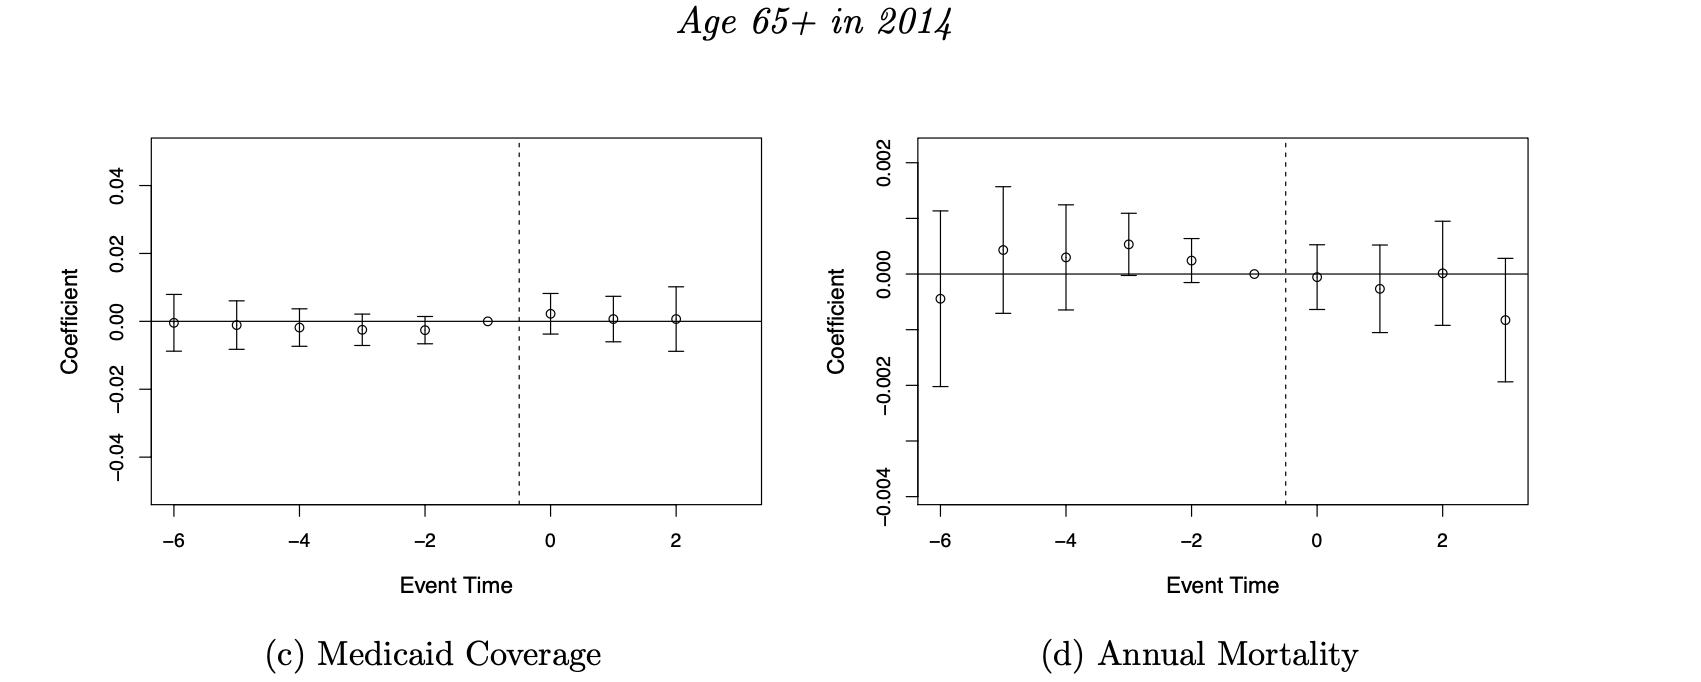
\includegraphics[scale=0.425]{./lecture_includes/placebo_medicaid}
	\end{figure}

\end{frame}

\begin{frame}{Main result}

\begin{itemize}

\item Finally they focus on the main result -- and there's more in the paper than I'm showing
\item Event study plots with same specification as the rest allowing us to look at the pre-trends and the post-treatment coefficients
\item If parallel trends holds, then the post-treatment coefficients are interpreted as ATT parameter estimates for each time period
\item The result alone isn't nearly as strong the result in combination with the rest, but it could still be wrong as parallel trends is ultimately not verfiable
\end{itemize}

\end{frame}



\begin{frame}{Near elderly mortality and Medicaid expansion}

	\begin{figure}
	\includegraphics[scale=0.3]{./lecture_includes/Miller_Medicaid4.png}
	\end{figure}

\end{frame}

\begin{frame}{Summarizing evidence and results}

\begin{itemize}
\item \textbf{Bite}: Increases in enrollment and reductions in uninsured support that there is adoption of the treatment
\item \textbf{Event studies}: Compelling graphics showing similarities between treatment and control
\item \textbf{Falsifications}: no effect on a similar group who isn't eligible
\item \textcolor{red}{Main results}: 9.2\% reduction in mortality among the near-elderly
\item \textcolor{red}{Mechanism}: ``The effect is driven by a reduction in disease-related deaths and grows over time.''
\end{itemize}

\end{frame}

\begin{frame}{Making event study}

\begin{itemize}
\item When there is only one treatment group and one comparison group, then you run a regression with an interaction of the treatment group dummy and the calendar year dummies (plus both separately)
\item You must drop $t-\tau$ as the baseline (e.g., $t-1$) and it must be $Y^0$ untreated comparisons (No Anticipation)
\item I have included in a do file that will do it for you either manually or using coefplot in \texttt{simple\_eventstudy.do} at the shared github labs directory
\end{itemize}

\end{frame}


\begin{frame}{Manually creating the event study}

	\begin{figure}
	\includegraphics[scale=0.20]{./lecture_includes/simple_eventstudy_manual}
	\end{figure}

\end{frame}




\begin{frame}{Creating the event study with Ben Jann's \texttt{coefplot}}

	\begin{figure}
	\includegraphics[scale=0.20]{./lecture_includes/simple_eventstudy.png}
	\end{figure}

\end{frame}




\begin{frame}{Parallel Trends}

\begin{itemize}

\item Of the three assumptions we discussed -- SUTVA and no treated control group, unconditional parallel trends, and no anticipation -- it's usually parallel trends we worry about
\item We discussed Event Studies
\item But we were focused on \emph{unconditional parallel trends} (i.e., no covariates), but is unconditional parallel trends plausible in your study?
\item Next we will explore when you think you need covariates -- why do you need them and how do you choose them?
\end{itemize}

\end{frame}




\section{Conditional Parallel Trends}

\subsection{Introducing Covariates}

\begin{frame}{Review}

\begin{itemize}
\item Diff in Diff is a quasi-experimental method that identifies the aggregate causal parameter, ATT, if:

	\begin{enumerate}
	\item Parallel trends holds
	\item And also no anticipation and if we use comparisons that aren't treated
	\end{enumerate}
	
\item But we worked with "unconditional parallel trends" which means this:

	$$ \bigg ( \textcolor{red}{E[Y^0_k|Post]} - E[Y^0_k|Pre] \bigg ) - \bigg ( E[Y^0_U|Post] - E[Y^0_U | Pre] \bigg )$$
	
\item This means that the \emph{average} treatment group potential outcome trends for our treatment group is the same as our control group

\end{itemize}

\end{frame}

\begin{frame}{Is Unconditional Parallel Trends Plausible?}

\begin{itemize}

\item But what if these two groups are different in ways that predict $Y^0$?

\item Let's say for instance that your study looks at an intervention that primarily effects cities, but your only control group are rural counties

\item These groups differ in a ways that might, depending on your study, not be plausibly suggesting they would've been on the same trends

\end{itemize}

\end{frame}

\begin{frame}{Conditional parallel trends}

\begin{itemize}

\item While it isn't required that two groups -- group $k$ and group $U$ -- be similar on observables for parallel trends to hold:

	\begin{enumerate}
	\item Remember, if treatment had been random, then they would have the average covariates
	\item And if they aren't, then you may need to provide more evidence that these differences are irrelevant
	\item So you should still check and see and if they aren't, you either adjust or have a good justification for why they're the same on trends in $E[Y^0]$ 
	\end{enumerate}
	
\item Including covariates weakens the unconditional parallel trends assumption by only requiring that units with similar covariate values, as opposed to everyone, follow similar counterfactual trends in $Y^0$
\item This is means switching out the \emph{unconditional parallel trends} assumption for the \emph{conditional parallel trends} assumption

\end{itemize}

\end{frame}

\begin{frame}{Why covariates?}

\begin{itemize}

\item The inclusion of covariates in diff-in-diff models is not about trying to find random variation in the treatment within values of the dimension of X
\item It is based on the claim that the inclusion of covariates is necessary to re-establish parallel trends
\item This is itself different than how covariates will be used in synthetic control, too
\end{itemize}

\end{frame}




\begin{frame}{Correcting the missingness problem}

\begin{eqnarray*}
\text{ATT} &=& E[\delta | D=1] \\
&=& E[Y^1-\textcolor{red}{Y^0} | D=1] \\
&=& E[Y^1 | D=1] - \textcolor{red}{E[Y^0|D=1]} \\
&=& E[Y | D=1] - \textcolor{red}{E[Y^0|D=1]} 
\end{eqnarray*}

\bigskip

We were always missing $Y^0$ values for the treatment group units, but parallel trends allowed us to impute it using the change in $[Y^0]|D=0]$ as a guide

\bigskip

But if that trend is not a good guide, then we cannot.  


\end{frame}


\begin{frame}{Conditional parallel trends}

The DiD equation yields:

\begin{eqnarray*}
\widehat{\delta} &=& \bigg ( E[Y_k|Post] - E[Y_k|Pre] \bigg ) - \bigg ( E[Y_U | Post ] - E[ Y_U | Pre] \bigg) \\
&=& \text{ATT} + \text{Non-parallel trends bias}
\end{eqnarray*}

\bigskip

If we believe that conditional on covariates, parallel trends holds, but only within values of $X$, then there are methods we can use that incorporate covariates into the DiD equation and unbiasedness returns

\bigskip 

The inclusion of covariates has particular regression specifications, plus there are alternative methods too, and we will review them

\end{frame}

\subsection{Choosing Covariates}

\begin{frame}{Picking covariates}

\begin{itemize}
\item You want to select confounders, which are baseline untreated covariates that predict both the treatment (and thus cause imbalance) but also the potential outcome, $Y^0$
\item You can use your common sense, logic, graphical models (i.e., DAGs) and familiarity of the subject 
	\begin{itemize}
	\item Our focus is on the covariates that are determinants of the outcome, and less so the treatment itself, because note our concern is the untreated potential outcome $Y^0$
	\end{itemize}
\item But you can also use some simple approaches that I'll suggest now
\end{itemize}

\end{frame}

\begin{frame}{Three ideas}

\begin{itemize}
\item Note that we are missing $\textcolor{red}{E[Y^0|D=1]}$, and so we want covariates that are highly predictive of that missing potential outcome -- problem is, it's missing
\item But what if we did this:
	\begin{enumerate}
	\item Drop all treated (post treatment treatment group) so that all outcomes are now $Y^0$ and regress that against candidate covariates, and select from there
	\item Drop post treatment treatment group units and drop the control units and regress $Y^0$ for the treated unit against baseline covariates and select from there
	\item Use $t-2$ and $t-1$ period, calculate $\Delta E[Y^0|D=1]$ and regress that against $t-1$ covariates and select from there
	\end{enumerate}
\item This is a more data driven procedure and is helping you figure out which covariates might be candidate confounders -- but note this still is not checking for imbalance
\end{itemize}

\end{frame}


\subsection{Checking for Imbalance}

\begin{frame}
    \frametitle{Covariate Balance and Parallel Trends}
    \begin{itemize}
        \item The parallel trends assumption is untestable but can be evaluated using observed covariates.
        \item Balance in key covariates helps assess whether treated and control groups would follow similar trends.
        \item Differences in demographics or economic conditions between groups can indicate violations of parallel trends.
        \item Use covariates that are unlikely to be affected by treatment to check balance.
    \end{itemize}
\end{frame}


\begin{frame}
    \frametitle{Baseline Covariates and Normalized Difference}
    \begin{itemize}
        \item Baseline covariates are measured before treatment ($t-1$). Check for balance between treatment and control groups.
        \item Report the averages of covariates for both groups in a table.
        \item The normalized difference is calculated as:
        $$ \text{Norm. Diff}_\omega = \frac{\overline{X}_{\omega,T} - \overline{X}_{\omega,C}}{\sqrt{(S_{\omega,T}^2 + S_{\omega,C}^2)/2}} $$
        \item The normalized difference measures imbalance; it should be less than 0.25 to avoid problematic imbalance Imbens and Rubin (2015).
    \end{itemize}
\end{frame}


\begin{frame}{Normalized Difference vs. Z-Score}
    \begin{itemize}
        \item \textbf{Normalized Difference:}
        \begin{itemize}
            \item Measures difference in group means (e.g., treatment vs. control)
            \item Interprets difference relative to pooled variance
            \item Used for comparing balance between groups
        \end{itemize}
        \vspace{0.5em}
        \item \textbf{Z-Score:}
        \begin{itemize}
            \item Measures distance of a single observation from the mean
            \item Expresses this distance in standard deviation units
            \item Used for assessing how unusual a single observation is
        \end{itemize}
        \vspace{0.5em}
        \item Both metrics standardize differences using standard deviation, making them unit-free and comparable across variables, but in our case we need to focus on differences between two groups, so we use the normalized difference and focus on a threshold of 0.25.
    \end{itemize}
\end{frame}


\begin{frame}
    \centering
    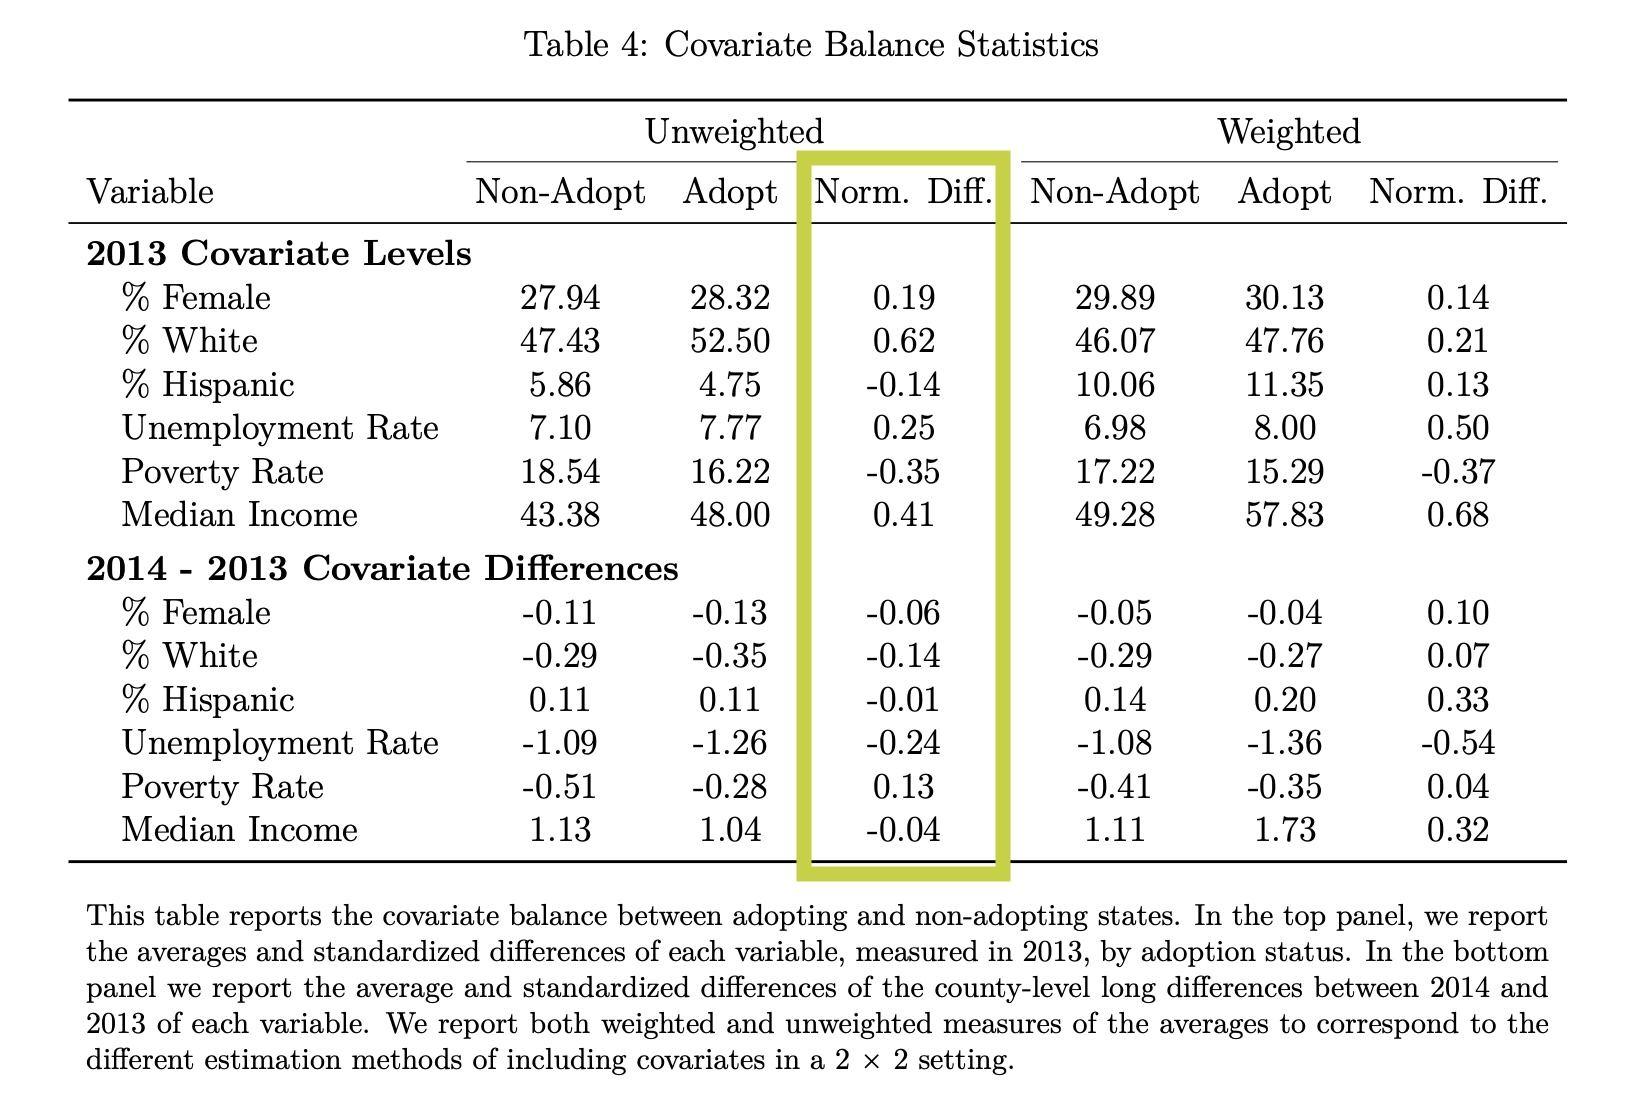
\includegraphics[width=0.9\textwidth]{./lecture_includes/table_jel_covariates.jpg}
\end{frame}

\begin{frame}
    \frametitle{Intuition for Checking Covariate Balance}
    \begin{itemize}
    \item Remember that confounders are variables that do two things
    	\begin{enumerate}
	\item $X \rightarrow D$. Confounders have different distributions in treatment than control and these balance checks are about seeing if that's true
	\item $X \rightarrow \Delta E[Y^0]$. But it's only a problem if the imbalance is on variables that also predict potential outcome trends, and we choose covariates based on things we think that's true
	\end{enumerate}
\item So you select covariates that you think are theoretically predictive of $Y^0$ trends, but then you check imbalance to see if they are differentially distributed 
    \end{itemize}
\end{frame}


\begin{frame}{Example: Murder}

\begin{itemize}
\item Say that there a set of cities pass gun law ordinances but smaller towns don't and you want to know its effect on homicides
\item Maybe as much as 80\% of homicides are in cities -- the homicides in small towns are rare, and the trends are probably pretty noisy and different
\item So you might think population size, could be a very important covariate to include or urbanization
\end{itemize}

\end{frame}





\begin{frame}{Three covariate DiD papers}

Three papers (though sometimes you see others) about covariate adjustment in DiD:
\begin{enumerate}
\item Abadie (2005) on semiparametric DiD -- reweights the comparison group part of the DID equation using a propensity score based on X
\item Heckman, Ichimura and Todd (1997) on outcome regression uses baseline X and control group only to impute the missing counterfactual $Y^0$ for treatment group units in a DiD equation
\item Sant'Anna and Zhou (2020) is double robust which means the method does both of these at the same time so that you don't have to choose between them
\end{enumerate}

\bigskip

We will discuss both of them and then compare their performance with the more straightforward fixed effects model

\end{frame}




\begin{frame}{Identification assumptions I: Data}

Assumption 1: Assume panel data or repeated cross-sectional data

\bigskip

Handling repeated cross-sectional data is possible but assumes stationarity which is a kind of stability assumption, but I'll use panel representation. 

\bigskip

Cross-sections will be potentially violated with changing sample compositions (e.g., the Napster example). 

\end{frame}

\begin{frame}{Identification assumptions II: Modification to parallel trends}

Assumption 2: Conditional parallel trends

\bigskip

Counterfactual trends for the treatment group are the same as the control group for all values of $X$

\begin{eqnarray*}
E[Y_1^0 - Y_0^0 | X, D=1] = E[Y^0_1 - Y^0_0 | X, D=0]
\end{eqnarray*}

\end{frame}

\begin{frame}{Identification assumptions III: Common support}

Assumption 3: Common support

\bigskip

For some $e>0$, the probability of being in the treatment group is greater than $e$ and the probability of being in the treatment group conditional on $X$ is $\leq1-e$. 

\bigskip

Heckman, et al doesn't use the propensity score so we need a more general expression of support

\end{frame}



\begin{frame}{Outcome regression}

This is the Heckman, et al. (1997) approach where the potential outcome evolution for the treatment group is imputed with a regression based only on $X_b$ for the control group \emph{only}

\bigskip

\begin{eqnarray*}
\widehat{\delta}^{OR} = \overline{Y}_{1,1} - \bigg [ \overline{Y}_{1,0} + \frac{1}{n^T} \sum_{i|D_i=1} ( \widehat{\mu}_{0,1}(X_i) - \widehat{\mu}_{0,0}(X_i)) \bigg ]
\end{eqnarray*}

where $\overline{Y}$ is the sample average of $Y$ among units in the treatment group at time $t$ and $\widehat{\mu}(X)$ is an estimator of the true, but unknown, $m_{d,t}(X)$ which is by definition equal to $E[Y_t|D=d,X=x]$.

\end{frame}




\begin{frame}{Outcome regression}

\begin{eqnarray*}
\widehat{\delta}^{OR} = \overline{Y}_{1,1} - \bigg [ \overline{Y}_{1,0} + \frac{1}{n^T} \sum_{i|D_i=1} ( \widehat{\mu}_{0,1}(X_i) - \widehat{\mu}_{0,0}(X_i)) \bigg ]
\end{eqnarray*}

\begin{enumerate}
\item Regress changes $\Delta Y$ on $X$ among untreated groups using baseline covariates only
\item Get fitted values of the regression using all $X$ from $D=1$ only.  Average those
\item Calculate change in this fitted $Y$ among treated with the average fitted values
\end{enumerate}

\end{frame}

\begin{frame}{Inverse probability weighting}

This is the Abadie (2005) approach where we use weighting

\begin{eqnarray*}
\widehat{\delta}^{ipw} = \frac{1}{E_N[D]} E \bigg [ \frac{D-\widehat{p}(X)}{1-\widehat{p}(X)} (Y_1-Y_0) \bigg ]
\end{eqnarray*}

where $\widehat{p}(X)$ is an estimator for the true propensity score. Reduces the dimensionality of $X$ into a single scalar.

\end{frame}

\begin{frame}{These models cannot be ranked}

\begin{itemize}
\item Outcome regression needs $\widehat{\mu}(X)$ to be correctly specified, whereas
\item Inverse probability weighting needs $\widehat{p}(X)$ to be correctly specified
\item It's hard to ``rank'' these two in practice with regards to model misspecification because each is inconsistent when their own models are misspecified
\item But what if you could do both of them at the same time and not pay for it?
\end{itemize}

\end{frame}

\begin{frame}{Double Robust DR}

\begin{itemize}
\item Doubly robust combines them to give us insurance; we now get two chances to be wrong, as opposed to just one
\item Two papers:
	\begin{enumerate}
	\item Chang (2020) incorporates DR with double/debiased ML
	\item Sant'Anna and Zhau (2020) is based on the IPW (Abadie 2005) and OR (Heckman, Ichimura and Todd 1997)
	\end{enumerate}
\item For now, I've prepped the latter, but will soon get Chang (2020) incorporated -- I just have been relying on Brigham Frandsen to teach the DML material
\end{itemize}

\end{frame}


\subsection{Double Robust}

\begin{frame}{Double Robust DiD}
\begin{eqnarray*}
\delta^{dr} = E \bigg [ \bigg ( \frac{D}{E[D]} -\frac{ \frac{p(X)(1-D)}{(1-p(X))} }{E \bigg [\frac{p(X)(1-D)}{(1-p(X))} \bigg ]} \bigg  )( \Delta Y - \mu_{0,\Delta}(X)) \bigg ]
\end{eqnarray*}

\begin{eqnarray*}
&&p(x): \text{propensity score model} \\
&& \Delta Y = Y_1 - Y_0 = Y_{post} - Y_{pre} \\
&& \mu_{d,\Delta} = \mu_{d,1}(X) - \mu_{d,0}(X), \text{ where } \mu(X) \text{ is a model for} \\
&& m_{d,t} = E[Y_t|D=d,X=x]
\end{eqnarray*}So that means $\mu_{0,\Delta}$ is just the control group's change in average $Y$ for each $X=x$

\end{frame}

\begin{frame}{Double Robust DiD}

\begin{eqnarray*}
\delta^{dr} = E \bigg [ \bigg ( \frac{D}{E[D]} -\frac{ \frac{p(X)(1-D)}{(1-p(X))} }{E \bigg [\frac{p(X)(1-D)}{(1-p(X))} \bigg ]} \bigg  )( \Delta Y - \mu_{0,\Delta}(X)) \bigg ]
\end{eqnarray*}

Notice how the model controls for $X$: you're weighting the adjusted outcomes using the propensity score

\bigskip

The reason you control for $X$ twice is because you don't know which model is right.  DR DiD frees you from making a choice without making you pay too much for it


\end{frame}

\begin{frame}{Efficiency}

\begin{itemize}
\item Authors exploit all the restrictions implied by the assumptions to construct semiparametric bounds
\item This is where the influence function comes in, which those who have studied the DID code closely may have noticed
\item One of the main results of the paper is that the DR DiD estimator is also DR for inference
\end{itemize}

\end{frame}

\subsection{Canonical TWFE with Additive Covariates}

\begin{frame}{Standard TWFE Model}

Consider our earlier TWFE specification:

\begin{eqnarray*}
Y_{it} = \alpha_1  + \alpha_2 T_t + \alpha_3 D_i +  \delta (T_i \times D_t)  + \varepsilon_{it}
\end{eqnarray*}

\bigskip

Just add in covariates then right?

\begin{eqnarray*}
Y_{it} = \alpha_1  + \alpha_2 T_t + \alpha_3 D_i  + \delta (T_i \times D_t) + \theta \cdot X_{it} + \varepsilon_{it}
\end{eqnarray*}

Sure! If you're willing to impose three \emph{more} assumptions

\end{frame}




\begin{frame}{Decomposing TWFE with covariates}

TWFE places restrictions on the DGP. Previous TWFE regression under assumptions 1-3 implies the following:

\bigskip

\begin{eqnarray*}
E[Y^1_1|D=1,X] = \alpha_1 + \alpha_2 + \alpha_3 + \delta + \theta X
\end{eqnarray*}

\bigskip

Conditional parallel trends implies

\small
\begin{eqnarray*}
&&E[Y^0_{1} - Y^0_{0}|D=1,X]= E[Y^0_{1} - Y^0_{0}|D=0,X] \\
&&E[Y^0_{1}|D=1,X] - E[Y^0_{0}|D=1,X]= E[Y^0_{1}|D=0,X] - E[Y^0_{0}|D=0,X] \\
&&E[Y^0_{1}|D=1,X] = E[Y^0_{0}|D=1,X] + E[Y^0_{1}|D=0,X] - E[Y^0_{0}|D=0,X] \\
&&E[Y^0_{1}|D=1,X] = E[Y_{0}|D=1,X] + E[Y_{1}|D=0,X] - E[Y_{0}|D=0,X] \\
\end{eqnarray*}


\end{frame}

\begin{frame}{Switching equation substitution}

Last line from the switching equation. This gives us:

\begin{eqnarray*}
E[Y^0_{1}|D=1,X] = \alpha_1  + \alpha_2 + \alpha_3 + \theta X
\end{eqnarray*}

Now compare this with our earlier $Y^1$ expression

\begin{eqnarray*}
E[Y^1_1|D=1,X] = \alpha_1 + \alpha_2 + \alpha_3 + \delta + \theta X
\end{eqnarray*}

We can define our target parameter, the ATT, now in terms of the fixed effects representation

\end{frame}


\begin{frame}{Collecting terms}

TWFE representation of our conditional expectations of the potential outcomes
\begin{eqnarray*}
&&E[Y^1_1|D=1,X] = \alpha_1 + \alpha_2 + \alpha_3 + \delta + \theta_1 X \\
&&E[Y^0_{1}|D=1,X] = \alpha_1  + \alpha_2 + \alpha_3 + \theta_2 X \\
\end{eqnarray*}

Substitute these into our target parameter

\begin{eqnarray*}
ATT &=& E[Y^1_1|D=1,X]  - E[Y^0_{1}|D=1,X]   \\
&&=(\alpha_1 + \alpha_2 + \alpha_3 + \delta + \theta_1 X) - ( \alpha_1  + \alpha_2 + \alpha_3 + \theta_2 X )\\
&&=\delta + (\theta_1 X - \theta_2 X)
\end{eqnarray*}

\bigskip

What if $\theta_1 X \neq \theta_2 X$?

\end{frame}

\begin{frame}{Assumption 4: Homogeneous treatment effects in X}


TWFE requires homogenous treatment effects in $X$ (i.e., the treatment effect is the same for all $X$)

\bigskip

If $X$ is sex, then effects are the same for males and females.

\bigskip

  If $X$ is continuous, like income, then the effect is the same whether someone makes \$1 or \$1 million.

\end{frame}

\begin{frame}{X-specific trends}

TWFE also places restrictions on covariate trends for the two groups too.  Take conditional expectations of our TWFE equation. 

\begin{eqnarray*}
E[Y_1|D=1] &=& \alpha_1 + \alpha_2 + \alpha_3 + \delta + \theta X_{11} \\
E[Y_0|D=1] &=& \alpha_1 + \alpha_3 + \theta X_{10} \\
E[Y_1|D=0] &=& \alpha_1 + \alpha_2 + \theta X_{01} \\
E[Y_0|D=0] &=& \alpha_1 + \theta X_{00}
\end{eqnarray*}


\end{frame}


\begin{frame}{X-specific trends}

Now take the DiD formula:

\begin{eqnarray*}
\delta^{DD} = &&\bigg ( (\alpha_1 + \alpha_2 + \alpha_3 + \delta + \theta X_{11} ) - (\alpha_1 + \alpha_3 + \theta X_{10} ) \bigg )- \\
&& \bigg ( (\alpha_1 + \alpha_2 + \theta X_{01}) - (\alpha_1 + \theta X_{00}) \bigg )
\end{eqnarray*}

\bigskip

Eliminating terms, we get:

\begin{eqnarray*}
\delta^{DD} = &&\delta + \\
&& (\theta X_{11} - \theta X_{10} ) - (\theta X_{01} - \theta X_{00} )
\end{eqnarray*}

\bigskip

Second line requires that trends in X for treatment group equal trends in X for control group.

\end{frame}


\begin{frame}{Assumption 5 and 6}

We need ``no X-specific trends'' for the treatment group (assumption 5) and comparison group (assumption 6)

\bigskip

\textbf{Intuition}: No X-specific trends means the evolution of potential outcome $Y^0$ is the same regardless of $X$. This would mean you cannot allow rich people to be on a different trend than poor people, for instance.

\bigskip

Without these six, in general TWFE will not identify ATT. 

\end{frame}

\begin{frame}{Why not both?}

\begin{itemize}
\item Let's review the problem.  What if you claim you need $X$ for conditional parallel trends?
\item You have three options:
	\begin{enumerate}
	\item Outcome regression (Heckman, et al. 1997) -- needs Assumptions 1-3
	\item Inverse probability weighting (Abadie 2005) -- needs Assumptions 1-3
	\item TWFE (everybody everywhere all the time) -- needs Assumptions 1-6
	\end{enumerate}
\item Problem is 1 and 2 need the models to be correctly specified
\item Let's look at a simulation
\end{itemize}

\end{frame}



\begin{frame}{Simulation}

\begin{itemize}

\item First we will look at the use of these estimators using a simulation named \texttt{covariates.do} and \texttt{covariates.R}

\item We will do it both with a single run, as that's faster, and then run a simulation of 1,000 simulated regenerated data (i.e., Monte Carlo simulation) to get a distribution

\item We will examine all four estimators: (1) OLS, (2) IPW, (3) OR and (4) DR

\end{itemize}

\end{frame}

\begin{frame}{Simulation}
    \centering
    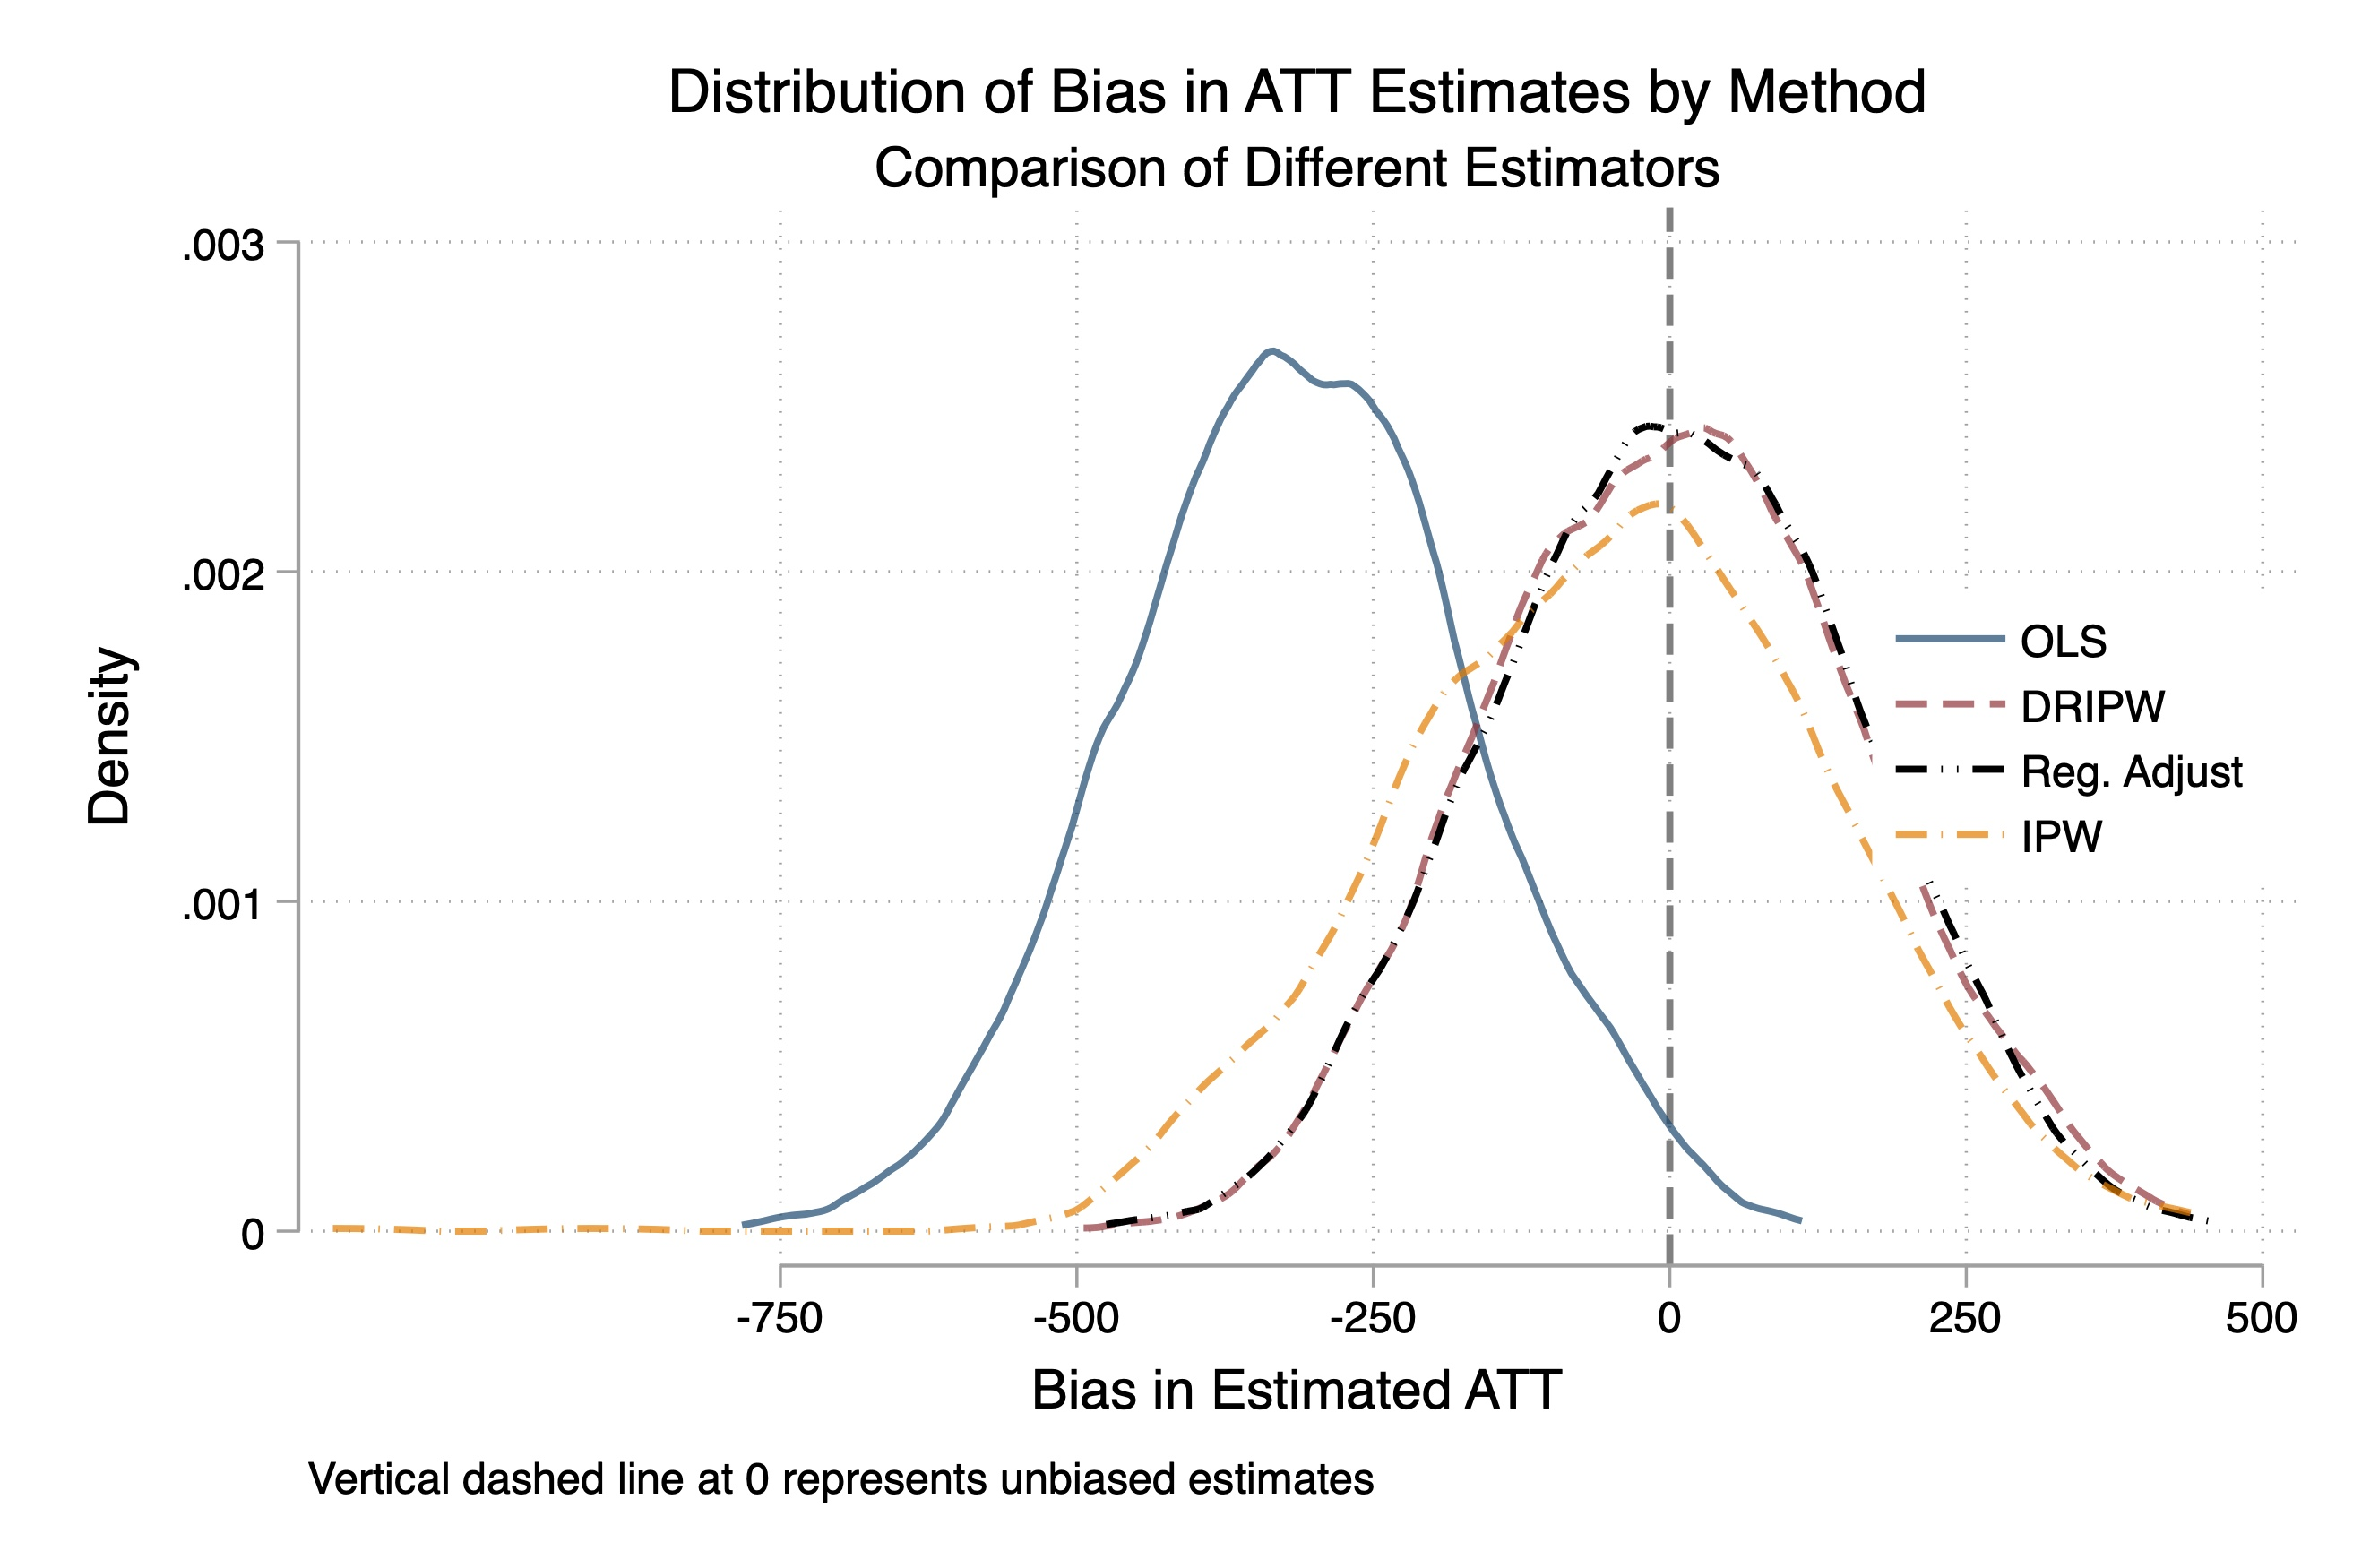
\includegraphics[width=0.6\textwidth]{./lecture_includes/covariates.jpg}
\end{frame}


\begin{frame}{R and Stata Code}

There is code in R and Stata (all DiD estimators are now beautifully arranged at a website hosted by Asjad Naqvi)
\begin{itemize}
\item Stata: \textbf{drdid}
\item R: \textbf{drdid}
\end{itemize}

\bigskip

\url{https://asjadnaqvi.github.io/DiD/docs/01_stata/}

\bigskip

Remember -- it's for 2x2 with covariates (i.e., one treatment group). 

\end{frame}


\end{document}


